\documentclass[tikz,border=5pt]{standalone}
\usepackage{times}
\usepackage{amsmath,amssymb}
\usetikzlibrary{positioning,fit,arrows.meta,backgrounds,shapes.geometric,calc,shadows,decorations.pathreplacing}

\begin{document}
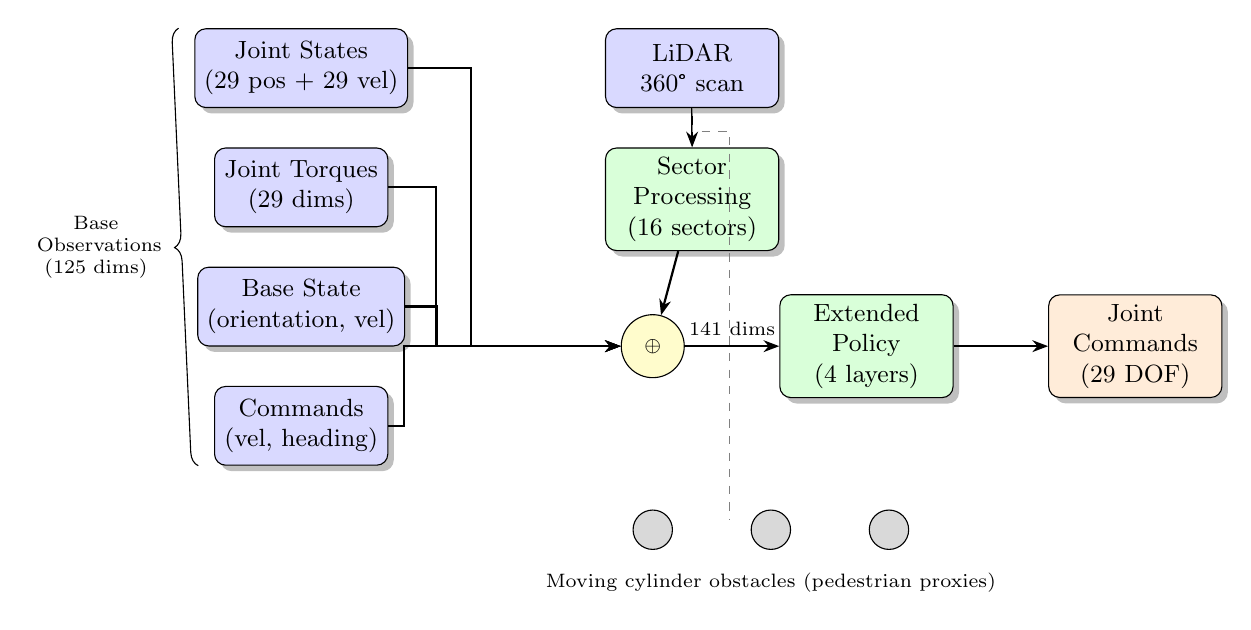
\begin{tikzpicture}[
    node distance=0.8cm and 1.2cm,
    box/.style={rectangle, draw, rounded corners, minimum height=1.0cm, minimum width=2.2cm, align=center, font=\small},
    sensor/.style={box, fill=blue!15, drop shadow},
    process/.style={box, fill=green!15, drop shadow},
    output/.style={box, fill=orange!15, drop shadow},
    concat/.style={circle, draw, fill=yellow!20, minimum size=0.8cm, font=\scriptsize},
    arrow/.style={-{Stealth[length=2mm]}, thick},
    label/.style={font=\scriptsize, align=center}
]

% Base locomotion observations (left column)
\node[sensor] (joints) {Joint States\\(29 pos + 29 vel)};
\node[sensor, below=0.5cm of joints] (torque) {Joint Torques\\(29 dims)};
\node[sensor, below=0.5cm of torque] (base) {Base State\\(orientation, vel)};
\node[sensor, below=0.5cm of base] (cmd) {Commands\\(vel, heading)};

% Brace for base observations
\node[left=0.3cm of joints, yshift=-1.5cm] (brace_label) {};
\draw[decorate, decoration={brace, amplitude=5pt, mirror}]
    ([xshift=-0.2cm]joints.north west) -- ([xshift=-0.2cm]cmd.south west)
    node[midway, left=0.3cm, label, text width=1.5cm] {Base\\Observations\\(125 dims)};

% LiDAR processing (middle-top)
\node[sensor, right=2.5cm of joints] (lidar_raw) {LiDAR\\360\textdegree{} scan};
\node[process, below=0.5cm of lidar_raw] (sector) {Sector\\Processing\\(16 sectors)};

% Arrow from lidar to sector
\draw[arrow] (lidar_raw) -- (sector);

% Concatenation node
\node[concat, below=0.8cm of sector, xshift=-0.5cm] (cat) {$\oplus$};

% Draw arrows to concatenation
\draw[arrow] (joints.east) -- ++(0.8,0) |- (cat);
\draw[arrow] (torque.east) -- ++(0.6,0) |- (cat);
\draw[arrow] (base.east) -- ++(0.4,0) |- (cat);
\draw[arrow] (cmd.east) -- ++(0.2,0) |- (cat);
\draw[arrow] (sector) -- (cat);

% Policy network
\node[process, right=1.2cm of cat] (policy) {Extended\\Policy\\(4 layers)};
\draw[arrow] (cat) -- (policy) node[midway, above, label] {141 dims};

% Output
\node[output, right=1.2cm of policy] (actions) {Joint\\Commands\\(29 DOF)};
\draw[arrow] (policy) -- (actions);

% Dynamic obstacles illustration (bottom)
\node[below=1.8cm of cat, xshift=1cm] (obstacles_label) {};
\draw[fill=gray!30] ([xshift=-1cm]obstacles_label) circle (0.25cm);
\draw[fill=gray!30] ([xshift=0.5cm]obstacles_label) circle (0.25cm);
\draw[fill=gray!30] ([xshift=2cm]obstacles_label) circle (0.25cm);
\node[below=0.3cm of obstacles_label, label, xshift=0.5cm] {Moving cylinder obstacles (pedestrian proxies)};

% Dotted line showing obstacle detection
\draw[dashed, gray] (lidar_raw.south) -- ++(0,-0.3) -| ([xshift=-1cm]obstacles_label);

\end{tikzpicture}
\end{document}
